\begin{Shaded}
\begin{Highlighting}[]
\KeywordTok{data}\NormalTok{(}
\NormalTok{  cogs,}
\NormalTok{  cogs_of_interest,}
\NormalTok{  string_eukaryotes,}
  \DataTypeTok{package =} \StringTok{"neurotransmissionevolution"}
\NormalTok{)}

\NormalTok{phyloTree <-}\StringTok{ }\KeywordTok{read.tree}\NormalTok{(}\StringTok{"../data/hybrid_tree_modified.nwk"}\NormalTok{)}
\end{Highlighting}
\end{Shaded}

Some minor data formatting is done before feeding it to geneplast

\begin{Shaded}
\begin{Highlighting}[]
\CommentTok{# formating cogdata column names for geneplast}
\NormalTok{cogs }\OperatorTok\StringTok{ }\KeywordTok{rename}\NormalTok{(}\DataTypeTok{protein_id =}\NormalTok{ string_id, }\DataTypeTok{ssp_id =}\NormalTok{ taxid) }\OperatorTok\StringTok{ }\KeywordTok{select}\NormalTok{(protein_id, ssp_id, cog_id)}

\CommentTok{# adding species names to taxid tree}
\NormalTok{phyloTree }\OperatorTok\StringTok{ }\KeywordTok{list_modify}\NormalTok{(}
  \DataTypeTok{tip.alias =}\NormalTok{ string_eukaryotes }\OperatorTok\StringTok{ }\NormalTok{string_name[}\KeywordTok{match}\NormalTok{(phyloTree[[}\StringTok{"tip.label"}\NormalTok{]], taxid)]}
\NormalTok{)}
\end{Highlighting}
\end{Shaded}

\hypertarget{geneplast}{%
\subsubsection{Geneplast}\label{geneplast}}

Geneplast's groot.preprocess function structures an \texttt{ogr} object
which the \texttt{groot} will perform the rooting on.

We retrieve the numeric root for the queried
\texttt{cogs\_of\_interest}, that is, orthologous groups pertaining to
neurotransmission genes.

\begin{Shaded}
\begin{Highlighting}[]
\NormalTok{roots <-}\StringTok{ }\KeywordTok{groot.get}\NormalTok{(ogr, }\DataTypeTok{what=}\StringTok{"results"}\NormalTok{) }\OperatorTok
\StringTok{  }\KeywordTok{rownames_to_column}\NormalTok{(}\StringTok{"cog_id"}\NormalTok{) }\OperatorTok
\StringTok{  }\KeywordTok{select}\NormalTok{(cog_id, Root) }\OperatorTok
\StringTok{  }\KeywordTok{rename}\NormalTok{(}\DataTypeTok{root =}\NormalTok{ Root)}

\KeywordTok{write_tsv}\NormalTok{(roots, }\StringTok{"geneplast_roots.tsv"}\NormalTok{)}
\end{Highlighting}
\end{Shaded}

\hypertarget{clade-names}{%
\paragraph{Clade names}\label{clade-names}}

\texttt{}\\
To ease our analysis, we query the NCBI Taxonomy API and try to find
most clade names automatically.

\begin{Shaded}
\begin{Highlighting}[]
\NormalTok{lineages <-}\StringTok{ }\KeywordTok{entrez_fetch}\NormalTok{(}
  \DataTypeTok{db      =} \StringTok{"taxonomy"}\NormalTok{,}
  \DataTypeTok{id      =}\NormalTok{ string_eukaryotes[[}\StringTok{"new_taxid"}\NormalTok{]],}
  \DataTypeTok{rettype =} \StringTok{"xml"}\NormalTok{,}
  \DataTypeTok{retmode =} \StringTok{"xml"}\NormalTok{,}
  \DataTypeTok{parsed  =} \OtherTok{TRUE}
\NormalTok{)}

\NormalTok{string_eukaryotes }\OperatorTok\StringTok{ }\KeywordTok{mutate}\NormalTok{(}
  \DataTypeTok{root        =}\NormalTok{ ogr}\OperatorTok{@}\NormalTok{tree}\OperatorTok{$}\NormalTok{tip.group[taxid],}
  \DataTypeTok{lineage_txt =} \KeywordTok{xpathSApply}\NormalTok{(lineages, }\StringTok{"//Lineage"}\NormalTok{, XML}\OperatorTok{::}\NormalTok{xmlValue)}
\NormalTok{)}
  
\NormalTok{roots_names <-}\StringTok{ }\NormalTok{string_eukaryotes }\OperatorTok
\StringTok{  }
\StringTok{  }\CommentTok{# splitting lienage text}
\StringTok{  }\KeywordTok{mutate}\NormalTok{(}\DataTypeTok{lineage_split =} \KeywordTok{strsplit}\NormalTok{(lineage_txt, }\StringTok{"; "}\NormalTok{)) }\OperatorTok
\StringTok{  }\KeywordTok{group_by}\NormalTok{(root) }\OperatorTok
\StringTok{  }
\StringTok{  }\CommentTok{# for each root, get all lineages intersections}
\StringTok{  }\CommentTok{# but also keep complete lineages for future use}
\StringTok{  }\KeywordTok{summarise}\NormalTok{(}\DataTypeTok{lineage =} \KeywordTok{Reduce}\NormalTok{(intersect, lineage_split) }\OperatorTok\StringTok{ }\NormalTok{list,}
            \DataTypeTok{lineage_list =}\NormalTok{ lineage_split }\OperatorTok\StringTok{ }\NormalTok{list) }\OperatorTok
\StringTok{  }
\StringTok{  }\CommentTok{# windowed lineage differences (window size = 3 -> curr, next, prev)}
\StringTok{  }\KeywordTok{mutate}\NormalTok{(}\DataTypeTok{downstream_diff =} \KeywordTok{mapply}\NormalTok{(setdiff,         lineage, }\KeywordTok{lead}\NormalTok{(lineage))) }\OperatorTok
\StringTok{  }\KeywordTok{mutate}\NormalTok{(}\DataTypeTok{upstream_diff   =} \KeywordTok{mapply}\NormalTok{(setdiff, downstream_diff,  }\KeywordTok{lag}\NormalTok{(lineage))) }\OperatorTok
\StringTok{  }
\StringTok{  }\CommentTok{# defaults to the furthest rank (i.e. the 1st one)}
\StringTok{  }\KeywordTok{mutate}\NormalTok{(}\DataTypeTok{clade_name =} \KeywordTok{map_chr}\NormalTok{(upstream_diff, }\DecValTok{1}\NormalTok{, }\DataTypeTok{.default =} \OtherTok{NA}\NormalTok{)) }\OperatorTok
\StringTok{  }
\StringTok{  }\CommentTok{# finding at what rank depth should mixed lineages be collapsed}
\StringTok{  }\KeywordTok{mutate}\NormalTok{(}\DataTypeTok{collapse_depth =}\NormalTok{ lineage }\OperatorTok\StringTok{ }\KeywordTok{map_int}\NormalTok{(length) }\OperatorTok{+}\StringTok{ }\DecValTok{1}\NormalTok{) }\OperatorTok
\StringTok{  }
\StringTok{  }\KeywordTok{group_by}\NormalTok{(root) }\OperatorTok
\StringTok{  }\CommentTok{# fallback_name is the collapsed lineage ranks}
\StringTok{  }\KeywordTok{mutate}\NormalTok{(}\DataTypeTok{fallback_name =}\NormalTok{ lineage_list }\OperatorTok
\StringTok{           }\NormalTok{flatten }\OperatorTok
\StringTok{           }\KeywordTok{map2_chr}\NormalTok{(collapse_depth, }\StringTok{`}\DataTypeTok{[}\StringTok{`}\NormalTok{) }\OperatorTok
\StringTok{           }\NormalTok{table }\OperatorTok
\StringTok{           }\KeywordTok{sort}\NormalTok{(}\OtherTok{TRUE}\NormalTok{) }\OperatorTok
\StringTok{           }\CommentTok{# names %>%}
\StringTok{           }\NormalTok{\{ }\KeywordTok{paste0}\NormalTok{(}\KeywordTok{names}\NormalTok{(.), }\StringTok{" ("}\NormalTok{, .,}\StringTok{")"}\NormalTok{) \} }\OperatorTok
\StringTok{           }\KeywordTok{paste0}\NormalTok{(}\DataTypeTok{collapse=}\StringTok{"; "}\NormalTok{)) }\OperatorTok
\StringTok{  }\KeywordTok{mutate}\NormalTok{(}\DataTypeTok{clade_name =} \KeywordTok{coalesce}\NormalTok{(clade_name, fallback_name)) }\OperatorTok
\StringTok{  }\KeywordTok{select}\NormalTok{(root, clade_name)}

\KeywordTok{write_tsv}\NormalTok{(roots_names, }\StringTok{"temp/temp_geneplast_clade_names.tsv"}\NormalTok{)}
\end{Highlighting}
\end{Shaded}

\hypertarget{plotting-roots}{%
\paragraph{Plotting roots}\label{plotting-roots}}

\texttt{}

\begin{Shaded}
\begin{Highlighting}[]
\NormalTok{tree_heatmap <-}\StringTok{ }\NormalTok{ogr}\OperatorTok{@}\NormalTok{orthoct }\OperatorTok
\StringTok{  }\KeywordTok{as_tibble}\NormalTok{(}\DataTypeTok{rownames =} \OtherTok{NA}\NormalTok{) }\OperatorTok
\StringTok{  }\KeywordTok{select}\NormalTok{(}\OperatorTok{-}\DecValTok{1}\NormalTok{)}

\NormalTok{phyloTreedata <-}\StringTok{ }\NormalTok{phyloTree }\OperatorTok
\StringTok{  }\KeywordTok{rotatePhyloTree}\NormalTok{(}\StringTok{"9606"}\NormalTok{) }\OperatorTok
\StringTok{  }\NormalTok{as_tibble }\OperatorTok
\StringTok{  }\KeywordTok{left_join}\NormalTok{(string_eukaryotes }\OperatorTok\StringTok{ }\KeywordTok{select}\NormalTok{(}\DataTypeTok{label =}\NormalTok{ taxid, ncbi_name, root)) }\OperatorTok
\StringTok{  }\NormalTok{as.treedata}

\NormalTok{p <-}\StringTok{ }\KeywordTok{ggtree}\NormalTok{(phyloTreedata, }\DataTypeTok{branch.length =} \StringTok{"none"}\NormalTok{, }\DataTypeTok{ladderize =}\NormalTok{ F) }\OperatorTok{+}
\StringTok{  }\KeywordTok{geom_tiplab}\NormalTok{(}\KeywordTok{aes}\NormalTok{(}\DataTypeTok{label =}\NormalTok{ ncbi_name), }\DataTypeTok{offset =} \DecValTok{1}\NormalTok{, }\DataTypeTok{hjust =} \DecValTok{0}\NormalTok{, }\DataTypeTok{align =}\NormalTok{ T) }\OperatorTok{+}
\StringTok{  }\KeywordTok{xlim}\NormalTok{(}\DecValTok{0}\NormalTok{,}\DecValTok{300}\NormalTok{)}

\KeywordTok{gheatmap}\NormalTok{(}
\NormalTok{  p,}
\NormalTok{  tree_heatmap,}
  \DataTypeTok{offset=}\DecValTok{50}\NormalTok{,}
  \DataTypeTok{width=}\DecValTok{5}\NormalTok{,}
  \DataTypeTok{font.size=}\DecValTok{2}\NormalTok{,}
  \DataTypeTok{colnames_angle=}\DecValTok{45}\NormalTok{,}
  \DataTypeTok{hjust=}\DecValTok{1}\NormalTok{,}
  \DataTypeTok{low =} \StringTok{"#DDDDDD"}\NormalTok{,}
  \DataTypeTok{high =} \StringTok{"#00AA44"}
\NormalTok{)}
\end{Highlighting}
\end{Shaded}

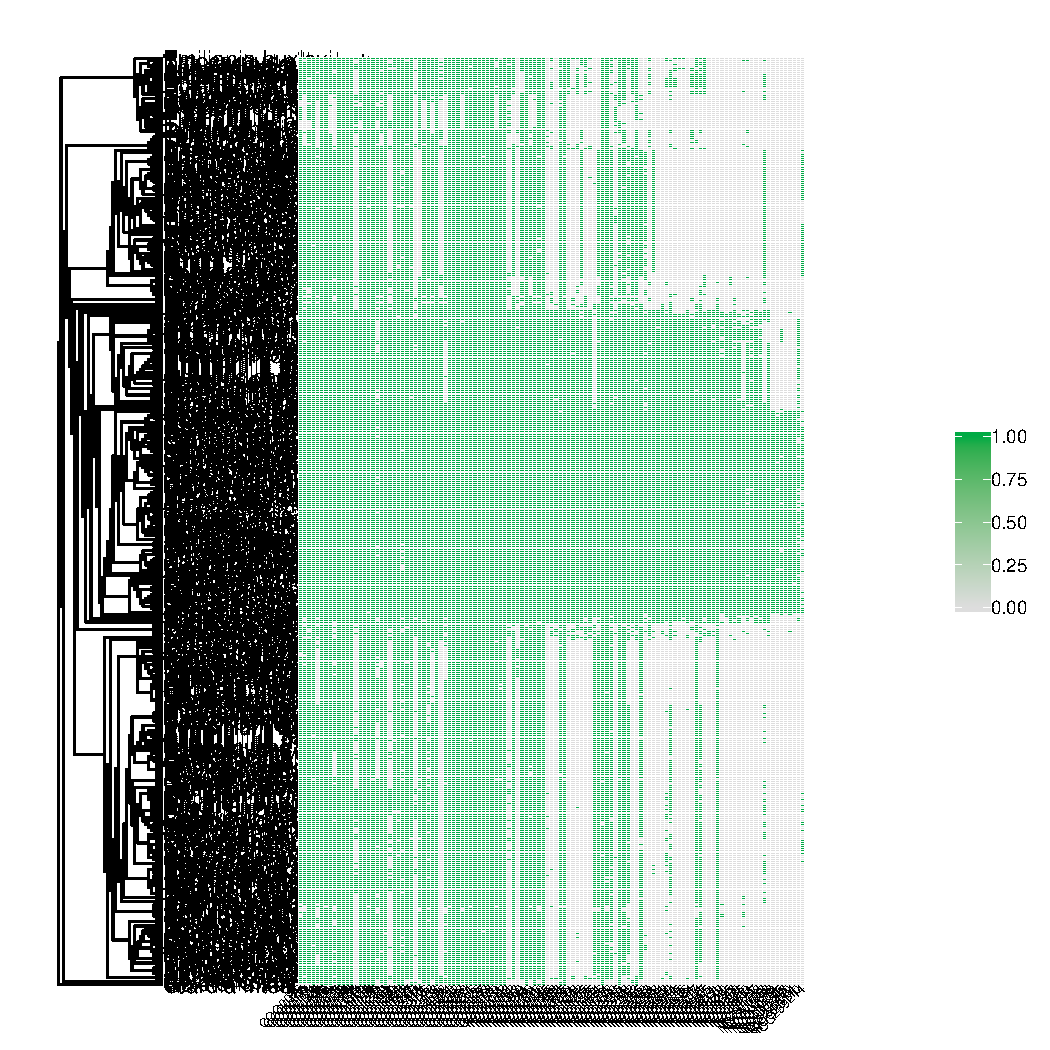
\includegraphics{figs/unnamed-chunk-9-1.pdf}
